%\documentclass[11pt,a4paper]{article}
%\usepackage{fullpage}
%\usepackage{beamerarticle}
%\documentclass[handout,xcolor=pdftex,dvipsnames,table]{beamer}
\documentclass[hyperref={unicode=true}]{beamer}

%\usepackage{pgfpages} 
%\pgfpagesuselayout{resize}[a4paper,border shrink=5mm,landscape] 

\usepackage[utf8]{inputenc}
\usepackage[russian]{babel}
\usepackage{../clrscode3e} 
%\usepackage[all]{xy}
\usepackage{colortbl}
%\usepackage{xcolor}
\usepackage{pstricks, pst-tree, pst-node}
\usepackage{epsfig}
\usepackage{multicol}
%\usepackage{listings}

\definecolor{orange}{cmyk}{0,0.52,1,0}

%\usepackage{beamerthemesplit}

\AtBeginSubsection[]
{
  \begin{frame}<beamer>{Раздел}
    \tableofcontents[currentsection,currentsubsection]
  \end{frame}
}


\newtheorem{rtheorem}{Теорема} 
\newtheorem{rconsequence}{Следствие} 
%default}
%themesplit}

\title{Суффиксные деревья}
\subtitle{Дискретный анализ 2012/13}
\author{Андрей Калинин, Татьяна Романова}
\date{26 ноября 2012\,г. }
\usetheme{default}
%\usefonttheme{serif}
\usefonttheme[onlymath]{serif}
%\usefonttheme{professionalfonts}
%\usetheme{default} 


\begin{document}

\frame{\titlepage}

%\section[Содержание]{}
\frame{\tableofcontents}

%\section{Литература}
\frame
{
  \frametitle{Литература}

  \begin{itemize}
  \item Дэн Гасфилд, <<Строки деревья и последовательности в алгоритмах:
    Информатика и вычислительная биология>>, 2003. Главы 5-6,
    <<Введение в суффиксные деревья>> и <<Построение суффиксных
    деревьев за линейное время>>, стр. 119--141.  
  \item E. Ukkonen. (1995). On-line construction of suffix trees.\\ http://www.cs.helsinki.fi/u/ukkonen/SuffixT1withFigs.pdf
  \end{itemize}
}


\section{Суффиксные деревья}

\subsection{Определение}

\frame{
  \frametitle{Определение}

  \begin{columns}
    \begin{column}{.7\textwidth}
  Суффиксное дерево $\mathbb{T}$ для $m$-символьной строки $S$:
  \begin{enumerate}
    \item Ориентированное дерево, имеющее ровно $m$ листьев,
      пронумерованных от $1$ до $m$.
    \item Каждая внутренняя вершина, отличная от корня, имеет не
      меньше двух детей. 
    \item Каждая дуга помечена непустой подстрокой строки $S$ (дуговая
      метка).
    \item Никакие две дуги, выходящие из одной вершины, не могут иметь
      меток, начинающихся с одинаковых символов. 
    \item Для каждого листа $i$ конкатенация меток от корня составляет
      $S[i..m]$. 
  \end{enumerate}
      \end{column}
    \begin{column}{.3\textwidth}
\onslide<2->{
  \pstree[treemode=R,levelsep=40pt,labelsep=2pt]{\Tdot}{
    \pstree{\Tdot}{\taput{$xa$}
      \pstree{\Tdot~{1}}{\taput{$bxac$}}
      \pstree{\Tdot~{4}}{\taput{$c$}}
    }
    \pstree{\Tdot}{\taput{$a$}
      \pstree{\Tdot~{2}}{\taput{$bxac$}}
      \pstree{\Tdot~{5}}{\taput{$c$}}
    }
    \pstree{\Tdot~{6}}{\taput{$c$}}
    \pstree{\Tdot~{3}}{\tbput{$bxac$}}
  } \\
~\\
~\\
      Дерево для строки $xabxac$.
}
\end{column}
\end{columns}
}

\frame{
  \frametitle{Терминальный символ}
  \begin{itemize}
    \item Суффиксное дерево нельзя построить для любой строки: если
      существует суффикс, совпадающий с префиксом другого суффикса, то
      не будет выполнено условие о количестве листьев. 
    \item Добавляется терминальный символ, который больше нигде в
      строке $S$ не содержится (будет обозначаться как $\$$). 
  \end{itemize}
}

\frame{
  \frametitle{Термины}
  \begin{itemize}
  \item Путевая метка вершины: конкатенация подстрок от корня до этой
    вершины в порядке прохождения соответствующих рёбер. 
  \item Строковая глубина вершины: количество символов в её путевой
    метке. 
  \item Если некоторый путь заканчивается внутри дуги $\langle u, v
    \rangle$, то путевая метка этого пути --- путевая метка $u$ с
    добавлением символов дуги $\langle u, v \rangle$ до места
    назначения. 
  \end{itemize}
}

\frame{
  \frametitle{Наивный алгоритм}
  \begin{itemize}
  \item Начиная со всей строки, последовательно вносить каждый суффикс
    в дерево. 
  \item  Время работы: для строки $S$ длиной $m$ --- $O(m^2)$.
  \item Существуют алгоритмы построения суффиксного дерева за $O(m)$
    в предположении ограниченного алфавита. 
  \end{itemize}
}

\subsection{Возможные приложения}

\frame{
  \frametitle{Поиск образца в тексте}
  \begin{columns}
    \begin{column}{.5\textwidth}
  \begin{itemize}
    \item Строится суффиксное дерево для текста.
    \item Ищется путь, совпадающий с образцом. 
      Если такого пути нет, то образец в текст не входит. 
      \item Если путь есть, то все листья поддерева --- вхождения.  
  \end{itemize}
\end{column}
\begin{column}{.5\textwidth}
  Поиск $aw$ в $awyawxawxz$:\\
~\\
~\\
~\\
  \pstree[treemode=R,levelsep=40pt,labelsep=2pt]{\Tdot}{
    \pstree{\Tdot}{\taput{$aw$}
      \pstree{\Tdot~{1}}{\taput{$y\cdots$}}
      \pstree{\Tdot}{\taput{$x$}
        \pstree{\Tdot~{7}}{\taput{$z\$$}}
        \pstree{\Tdot~{4}}{\tbput{$a\cdots$}}
      }
    }
  }
\end{column}
\end{columns}
}

\frame{
  \frametitle{Свойства}
  \begin{itemize}
  \item Если суффиксное дерево строится за линейное время, то время
    поиска $O(m+n)$, как и для ранее рассмотренных 
    алгоритмов. 
  \item Но: предварительная обработка $O(m)$, время поиска $O(n)$
    (в других алгоритмах было наоборот). 
  \item При обработке большого количества образцов (заранее неизвестного
    количества) можно выполнять поиск каждого из них в заранее
    известном тексте за время, зависящее только от длины образца!
  \end{itemize}
}

\frame{
  \frametitle{Ещё приложения}
  \begin{itemize}
  \item Нахождение общих подстрок для двух и более строк. 
  \item Компрессия данных. 
  \item Нечёткий поиск. 
  \item Выделение повторяющихся фрагментов. 
  \end{itemize}
}

\section{Алгоритм Укконена}

\subsection{Общее описание}

\frame{
  \frametitle{Неявные суффиксные деревья}

  Неявное суффиксное дерево может быть получено из суффиксного дерева
  строки $S$: 
  \begin{enumerate}
    \item удалением всех вхождений терминального символа;
    \item затем удалением всех дуг без меток; 
    \item затем удалением всех вершин, имеющих меньше двух детей (кроме
      корня). 
  \end{enumerate}

  $\mathbb{T}_i$ --- неявное суффиксное дерево для строки $S[1..i]$.
}

\frame{
  \frametitle{Неявное суффиксное дерево}

  \begin{columns}
    \begin{column}{.5\textwidth}
      Суффиксное дерево для $xabxa\$$:\\~\\
  \pstree[treemode=R,levelsep=40pt,labelsep=2pt]{\Tdot}{
    \pstree{\Tdot}{\taput{$xa$}
      \pstree{\Tdot~{1}}{\taput{$bxa\$$}}
      \pstree{\Tdot~{4}}{\taput{$\$$}}
    }
    \pstree{\Tdot}{\taput{$a$}
      \pstree{\Tdot~{2}}{\taput{$bxa\$$}}
      \pstree{\Tdot~{5}}{\taput{$\$$}}
    }
    \pstree{\Tdot~{6}}{\taput{$\$$}}
    \pstree{\Tdot~{3}}{\tbput{$bxa\$$}}
  }
  \end{column}
  \begin{column}{.5\textwidth}
    Неявное суффиксное дерево для $xabxa$:\\~\\~\\~\\~\\
  \pstree[treemode=R,levelsep=80pt,labelsep=2pt]{\Tdot}{
    \pstree{\Tdot~{1}}{\taput{$xabxa$}}
    \pstree{\Tdot~{2}}{\taput{$abxa$}}
    \pstree{\Tdot~{3}}{\tbput{$bxa$}}
  }\\~\\~\\~\\
\end{column}

  \end{columns}
}

\frame{
  \frametitle{Алгоритм Укконена}
  \begin{itemize}
  \item Последовательно строит неявные деревья $\mathbb{T}_i$ для
    каждого префикса $S[1..i]$.
  \item Настоящее суффиксное дерево $\mathbb{T}$ можно получить из
    $\mathbb{T}_m$ построив следующее неявное дерево для строки с терминальным
    символом. 
  \item Сначала рассмотрим метод построения дерева за $O(m^3)$, потом
    улучшим. 
  \end{itemize}
}

\frame{
  \frametitle{Общий вид алгоритма}

  \begin{codebox}
    \li Построить дерево $\mathbb{T}_1$ (одна дуга с $S(1)$).
    \li \For $i \gets 1$ \To $m-1$ \Comment Фаза $i+1$
    \li \Do \For $j \gets 1$ \To $i+1$ \Comment Продолжение $j$
    \li \Do Найти в $\mathbb{T}_i$ путь с меткой $S[j..i]$.
    \li Если нужно, продолжить путь, добавив символ $S(i+1)$.
    \zi \Comment Тогда строка $S[j..i+1]$ будет содержаться в дереве.
    \End 
    \li \Comment В результате получится дерево $\mathbb{T}_{i+1}$\End
  \end{codebox}
}

\frame{
  \frametitle{Правила продолжения суффиксов}
  $\beta = S[j..i]$ --- суффикс $S[1..i]$. Алгоритм находит конец
  пути $\beta$ и продолжает его так, чтобы $\beta S(i+1)$ так же
  входил в дерево. 
  \pause
  \begin{enumerate}
  \item Путь $\beta$ кончается в листе: нужно добавить $S(i+1)$ в
    хвост листовой дуги этого пути. 
   \pause
  \item Ни один путь из конца строки $\beta$ не начинается символом
    $S(i+1)$, но хотя бы один путь оттуда имеется: нужно создать новую
    листовую дугу, помеченную $S(i+1)$ и указать новому листу номер
    $j$. 
    \pause
  \item Есть некоторый путь от конца строки $\beta$, начинающийся
    символом $S(i+1)$: ничего делать не надо, строка $\beta S(i+1)$ уже есть в дереве. 
  \end{enumerate}
}

\frame{
  \frametitle{Время работы}
  \begin{itemize}
    \item $m$ фаз. 
    \item В каждой $i$-й фазе $i+1$ продолжение. 
    \item Каждое продолжение --- поиск от корня окончания пути
      $\beta$, максимум $|\beta|$ операций. 
    \item Само продолжение --- константное время. 
    \item Следовательно, время работы $O(m^3)$.
      \pause
    \item Нужно найти более быстрый метод определения места следующего
      продолжения (переход от $S[j..i+1]$ к $S[j+1..i+1]$).
  \end{itemize}
}

\subsection{Ускорение до $O(m^2)$}

\frame{
  \frametitle{Создание суффиксных связей}
  \begin{rtheorem}
    Если в продолжении $j$ фазы $i+1$ добавляется новая внутренняя
    вершина $v$ с путевой меткой $x\alpha$, то путь с меткой $\alpha$
    либо уже заканчивается в какой-то внутренней вершине дерева, либо
    новая вершина в конце $\alpha$ будет создана в продолжении $j+1$
    той же фазы $i+1$.
  \end{rtheorem}
  \begin{proof}
    \begin{itemize}
      \item Выполняется правило 2, следовательно существует путь
        $x\alpha c$, где $c\neq S(i+1)$.
      \item Следовательно, уже существует путь $\alpha c$.
      \item Если существует путь $\alpha d, d\neq c$, то нужная вершина в
        дереве уже есть. Иначе она создастся при
        добавлении $\alpha S(i+1)$, т.е. на следующем продолжении. 
    \end{itemize}
  \end{proof}
}

\frame{
  \frametitle{Следствия}
  \begin{enumerate}
    \item В алгоритме Укконена любая вновь созданная вершина получит
суффиксную связь при выполнении следующего продолжения.
    \item В любом неявном суффиксном дереве $\mathbb{T}_i$ если
      внутренняя вершина $v$ имеет путевую метку $x\alpha$, то
      найдётся вершина $s(v)$ дерева $\mathbb{T}_i$ с путевой меткой
      $\alpha$. 
  \end{enumerate}
}

\frame{
  \frametitle{Переходы по суффиксным связям при построении
    $\mathbb{T}_{i+1}$}
  \begin{itemize}
  \item При последовательном выполнении алгоритма в конце
    $S[j..i]$ выполняем продолжение и затем нужно попасть в конец
    $S[j+1..i]$.
  \item Конец полной строки $S[1..i]$ можно всегда хранить (это лист,
    соответствующий самому длинному пути). 
  \item Допустим, $S[1..i]=x\alpha$ и $\langle v, 1 \rangle$ --- дуга
    дерева, входящая в лист~1; нужно найти конец $S[2..i]=\alpha$.
    \item Если $v$ --- корень, то нужно выполнить поиск прямым способом. 
    \item Если же $v$ --- внутренняя вершина, и путь $\langle v,1
      \rangle$ помечен $\gamma$, то нужно пройти к $s(v)$ и оттуда
      проследовать вдоль $\gamma$, конец этого пути будет концом и $\alpha$.
  \end{itemize}

}

\frame{
  \frametitle{$j$-ое продолжение}
\begin{columns}
\begin{column}{.4\textwidth}
\includegraphics[scale=1.0]{suf-tree.1.eps}
\end{column}
\begin{column}{.6\textwidth}
 \begin{enumerate}
 \item Поднимаемся вверх не более чем на одну дугу (с меткой
   $\gamma$) к вершине $v$.
 \item Переходим по суффиксной связи в $s(v)$.
\item Опускаемся по пути, определяемому подстрокой $\gamma$.
 \end{enumerate}
\end{column}
\end{columns}
}

\frame{
   \frametitle{Алгоритм отдельного продолжения}
   Продолжение $j\geq 2$ фазы $i+1$:
   \begin{enumerate}
     \item Найти в конце строки $S[j-1..i]$ или выше первую вершину~$v$,
     которая либо имеет суффиксную связь, либо является
     корнем. $\gamma$ --- строка между $v$ и концом $S[j-1..i]$,
     возможно, пустая. 
     \item Если $v$ --- не корень, пройти в $s(v)$ и спуститься оттуда
       по пути $\gamma$. Если $v$ --- корень, пройти по пути
       $S[j..i]$.
     \item Выполнить правила продолжения (обеспечить вхождение
       $S[j..i+1]$).
     \item Если в продолжении $j-1$ была создана вершина $w$ для $x\alpha$, то
       связать её суффиксной связью с концом строки $\alpha$,
       найденном в текущем продолжении. 
   \end{enumerate}
   Первое продолжение всегда начинается с сохранённого окончания $S[1..i]$.
}

\frame{
  \frametitle{Что дало использование суффиксных связей?}
  \begin{itemize}
  \item Явное практическое улучшение. 
  \item Однако, оценка худшего случая не изменилась --- одна фаза за
    $O(m^2)$, полное выполнение --- $O(m^3)$.
  \item Продолжаем дальше: избавляемся от ненужных сравнений
    символов, для поиска пути можно перейти от времени
    пропроциональному $|\gamma|$ к времени, пропорциональному
    количеству вершин на пути. 
  \end{itemize}
}

\frame{
  \frametitle{Прыжок по счётчику}
\begin{columns}
\begin{column}{.55\textwidth}
\includegraphics[scale=1.0]{suf-tree.2.eps}
\end{column}
\begin{column}{.45\textwidth}
\begin{itemize}
\item Пусть $g=|\gamma|$ и $g'$ --- количество символов на дуге
  выходящей из $s(v)$ и помеченной первым символом $\gamma$.
\item Если $g'<g$, то остальные символы дуги просматривать не надо,
  можно сразу перейти к следующей вершине.
\end{itemize}
\end{column}
\end{columns}
}

\frame{
  \frametitle{Вершинная глубина}
  \begin{itemize}
  \item Полное время прохода по пути пропрционально числу вершин, а не
    символов. 
  \item Вершинная глубина узла $v$ --- число вершин на пути до неё от
    корня, $h(v)$. 
  \item Текущая вершинная глубина --- глубина последней по времени
    вершины, посещённой алгоритмом. 
  \end{itemize}
}

\frame{
  \frametitle{Вершинная глубина суффиксной связи}
\begin{columns}
\begin{column}{.55\textwidth}
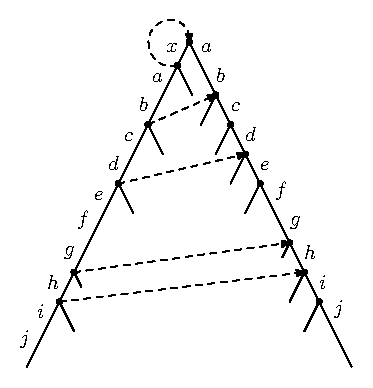
\includegraphics[scale=1.0]{suf-tree.4.eps}
\end{column}
\begin{column}{.45\textwidth}
  \begin{rtheorem}
    Пусть $\langle v, s(v) \rangle$ --- суффиксная связь, проходимая
    при выполнении алгоритма. В этот момент $h(v)\leq h(s(v))+1$.
  \end{rtheorem}
\end{column}
\end{columns}
}

\frame{
  \frametitle{Время выполнения одной фазы}
  \begin{rtheorem}
    При использовании прыжков по счётчику любая фаза алгоритма
    Укконена занимает время $O(m)$.
  \end{rtheorem}
  \begin{proof}
    \begin{enumerate}
    \item Подъём по дуге может уменьшить текущую вершиную глубину на
      1, проход по суффиксной связи так же может уменьшить её не более
      чем на 1, а каждая дуга при спуске увеличивает вершинную глубину. 
    \item Тем самым, за всю фазу текущая глубина уменьшается не более
      $2m$ раз. 
    \item Отсюда, т.к. глубина любой вершины меньше $m$,  приращение
      текущей глубины не превосходит $3m$. 
    \end{enumerate}
  \end{proof}
}

\frame{
  \frametitle{Время выполнения алгоритма}
  \begin{itemize}
  \item Суффиксные связи в алгоритме Укконена обеспечивают время работы
    $O(m^2)$.
  \item Если хранить строки на дугах, то требуется объём памяти
    $\Theta(m^2)$.
  \item Для перехода к линейному алгоритму требуется иное
    представление данных в дереве. 
  \end{itemize}
}

\subsection{Ускорение до $O(m)$}

\frame{
  \frametitle{Сжатие дуговых меток}
  Вместо выписывания подстрок достаточно хранить пару индексов,
  определяющую начальную и конечную позиции этой подстроки в $S$,
  откуда, имея доступ к $S$, всегда можно получить нужные символы. \\
~\\
  Например, $S=abcdefabcuvw$\\
~\\
~\\
  \begin{columns}
    \begin{column}{.5\textwidth}
      \pstree[treemode=R,levelsep=60pt,labelsep=2pt]{\Tdot}{
        \pstree{\Tdot}{\taput{$abc$}
          \pstree{\Tdot}{\taput{$uvw$}}
          \pstree{\Tdot}{\tbput{$def$}}
        }
        \pstree{\Tdot}{\tbput{$bc$}
          \pstree{\Tdot}{\taput{$uvw$}}
          \pstree{\Tdot}{\tbput{$def$}}
        }
      }
  \end{column}
  \begin{column}{.5\textwidth}
      \pstree[treemode=R,levelsep=60pt,labelsep=2pt]{\Tdot}{
        \pstree{\Tdot}{\taput{1,3}
          \pstree{\Tdot}{\taput{10,12}}
          \pstree{\Tdot}{\tbput{4,6}}
        }
        \pstree{\Tdot}{\tbput{2,3}
          \pstree{\Tdot}{\taput{10,12}}
          \pstree{\Tdot}{\tbput{4,6}}
        }
      }

  \end{column}
  \end{columns}

}

\frame{
  \frametitle{Третье правило завершает фазу}

  \begin{itemize}
  \item Правило 3: если уже существует путь $S[j..i+1]$, то
    ничего делать не надо. 
  \item Однако, если есть путь $S[j..i+1]$, то есть $S[j+1..i+1]$ и
    т.п. 
  \item Следовательно, для всех следующих продолжений будет
    выполняться третье правило. 
  \item Таким образом, фазу можно заканчивать при первом выполнении
    третьего правила. 
  \end{itemize}
}

\frame{
  \frametitle{Листья остаются листьями}

  \begin{itemize}
    \item Если был создан лист с меткой $j$, то он останется листом
      вплоть до окончания алгоритма. 
    \item То есть, во всех следующих фазах для этого продолжения будет
      применяться первое правило (дописать символ в конец листовой
      дуги). 
    \item Тем самым, можно помечать все листовые дуги не конкретным
      индексом, а глобальным индексом <<текущего окончания строки>>
      $e$, который увеличивать в начале фазы, выполняя
      неявно все продолжения по первому правилу. 
  \end{itemize}
}

\frame{
  \frametitle{Общая идея линейного алгоритма}
  \begin{itemize}
    \item Запоминается число $l$ --- последний лист, созданный на
      $i$-й фазе. 
    \item Выполнение всех первых правил происходит неявно, увеличивая
      $e$. 
    \item  Каждая фаза: последовательное применение второго правила
      (увеличивающее $l$) до первого срабатывания третьего правила. 
    \item Тем самым алгоритм превращается в последовательное
      выполнение правил номер 2. 
  \end{itemize}
}

\frame{
  \frametitle{Алгоритм одной фазы $i+1$}
  \begin{enumerate}
    \item $e \gets i+1$
    \item Вычислить все последовательные продолжения от $l$ до
      $r$, где применяется третье правило или до конца фазы. 
    \item $l \gets r$
  \end{enumerate}
}

\frame{
  \frametitle{Линейность алгоритма}
  \begin{rtheorem}
    Используя суффиксные связи и все улучшения, алгоритм Укконена
    строит неявные суффиксные деревья от $\mathbb{T}_1$ до
    $\mathbb{T}_m$ за полное время $O(m)$.
  \end{rtheorem}
  \begin{proof}
    \begin{enumerate}
    \item ${j'}$ --- продолжение, явно выполняемое
      алгоритмом. ${j'}$ не убывает и не изменяется при
      переходе от фазы к фазе, фаз $m$ и ${j'}\leq m$,
      следовательно количество продолжений не более $2m$.
    \item При этом текущая вершинная глубина не изменяется при
      переходе от фазы к фазе, то и максимальное количество прыжков
      для всех фаз имеет порядок $O(m)$.
    \end{enumerate}
  \end{proof}
}

\frame{
  \frametitle{Создание настоящего суффиксного дерева}
  \begin{itemize}
  \item Нужно добавить терминальный символ (выполнить ещё одну фазу). 
  \item Заменить глобальный индекс $e$ числом $m$.
  \item Тем самым, алгоритм Укконена строит настоящее суффиксное
    дерево для $S$ и всего его суффиксные связи за время $O(m)$.
  \end{itemize}
}


\end{document}
    
